%%%%%%%%%%%%%%%%%%%%%%%%%%%%%%%%%%%%%%%%%%%%%%%%%%%%%%%%%%%%%%%%%%%%%%%%%%%%%%%%
%2345678901234567890123456789012345678901234567890123456789012345678901234567890
%        1         2         3         4         5         6         7         8

% Key links for ICRA2020
% CFP: https://www.icra2020.org/call-for-papers
% PaperPlaza: https://ras.papercept.net/conferences/scripts/start.pl
% Author Guidelines: http://ras.papercept.net/conferences/support/tex.php

\documentclass[letterpaper, 10 pt, conference]{ieeeconf}
%\documentclass[a4paper, 10pt, conference]{ieeeconf}

% This command is only needed if you want to use the \thanks command
\IEEEoverridecommandlockouts

\overrideIEEEmargins

%In case you encounter the following error:
%Error 1010 The PDF file may be corrupt (unable to open PDF file) OR
%Error 1000 An error occurred while parsing a contents stream. Unable to analyze the PDF file.
%This is a known problem with pdfLaTeX conversion filter. The file cannot be opened with acrobat reader
%Please use one of the alternatives below to circumvent this error by uncommenting one or the other
%\pdfobjcompresslevel=0
%\pdfminorversion=4

% See the \addtolength command later in the file to balance the column lengths
% on the last page of the document

\usepackage{amsmath,amssymb,bm}
\usepackage{textcomp,gensymb}
\usepackage{tabularx,booktabs}
\usepackage{array,subcaption}
\let\labelindent\relax
\usepackage{enumitem}
\usepackage{graphicx}
\usepackage{hyperref}
\usepackage{color,soul}

\captionsetup[table]{
    justification=centerlast,
    textfont=small,
}

\graphicspath{{figures/}}

% Set a style for an entire table row
\newcolumntype{$}{>{\global\let\currentrowstyle\relax}}
\newcolumntype{^}{>{\currentrowstyle}}
\newcommand{\rowstyle}[1]{\gdef\currentrowstyle{#1}%
    #1\ignorespaces
}

% Some small icons we use in the text
\newcommand{\com}{\,
\includegraphics[width=9pt]{ico-com}\,}
\newcommand{\hinge}{\,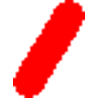
\includegraphics[width=9pt]{ico-hinge}\,}
\newcommand{\motor}{\,
\includegraphics[width=9pt]{ico-motor}\,}

\usepackage{lipsum}

\title{
    \LARGE \bf%
    A Reduced-Order Approach to Assist with Reinforcement Learning for Underactuated Robotics
}

\author{
    J\'er\'emy Augot$^{1,2}$, Aaron J. Snoswell$^{2}$ and Surya P. N. Singh$^{2}$
    % <-this % stops a space
    \thanks{
        $^{1}$Ecole CentraleSup\'elec, Paris, France
    }%
    \thanks{
        $^{2}$The Robotics Design Lab at The University of Queensland, Brisbane, Australia.  
        %{\texttt{\{j.augot, aaron.snoswell, spns\}@uq.edu.au}}
    }%
}

\begin{document}

\maketitle
\thispagestyle{empty}
\pagestyle{empty}

%%%%%%%%%%%%%%%%%%%%%%%%%%%%%%%%%%%%%%%%%%%%%%%%%%%%%%%%%%%%%%%%%%%%%%%%%%%%%%%%
\begin{abstract}


Compliant underactuated robots are a promising design strategy due to their electromechanical simplicity; however, their control can be rather complex as these robots can be difficult to model.  Recent Deep Reinforcement Learning and simulation methods together could help overcome this bottleneck.  However, these robots tend to exhibit spare rewards and thus making the control policy exploration non-trivial and highly variable.    

We use the intuition that an underactuated system has correlations between states and thus a reduced order representation might help focus control policy exploration process.   To help study this topic, we introduce \emph{The Jitterbug Task} of controlling a compliant legged toy robot with just a single motor across a field and to a location.    

Through this study we find that reduced order models can have similar (reward) performance, yet empirically have less training variance and slightly better learning rates.  

\end{abstract}

%%%%%%%%%%%%%%%%%%%%%%%%%%%%%%%%%%%%%%%%%%%%%%%%%%%%%%%%%%%%%%%%%%%%%%%%%%%%%%%%
\section{Introduction}

As robots become increasingly variable and compliant they become more capable, and complex.
Underactuated robots, for example, provide great design freedom, yet their adoption has been limited by the need for manual controller designs.

Deep Reinforcement Learning methods offer automated tools for robotic control by identifying a policy that maximizes the expected sum of rewards \cite{henderson2018deep}.
This has been extended to continuous control domains via algorithms such as the Deep Deterministic Policy Gradient (DDPG) \cite{DDPG}, Proximal Policy Optimization (PPO) \cite{PPO}, Soft Actor-Critic (SAC) \cite{SAC}, and Twin Delayed Deep Deterministic (TD3) \cite{TD3}.
The power of these methods comes, in part, from the high-dimensional, nonlinear function approximation of both the policy and the expected value by neural networks.
The dimensionality of these rich representations also presents challenges, particularly for sample collection, stability, and convergence \cite{Islam2017}.
Reducing the order seems a natural approach to addressing these challenges, but doing so directly requires carefully defining suitable (state-space) features as the aforementioned methods are sensitive to the chosen representation \cite{bhatnagar2009convergent}.  

\begin{figure}[t]
    
    \centering
    
    \begin{minipage}[b]{0.49\linewidth}
        \centering
        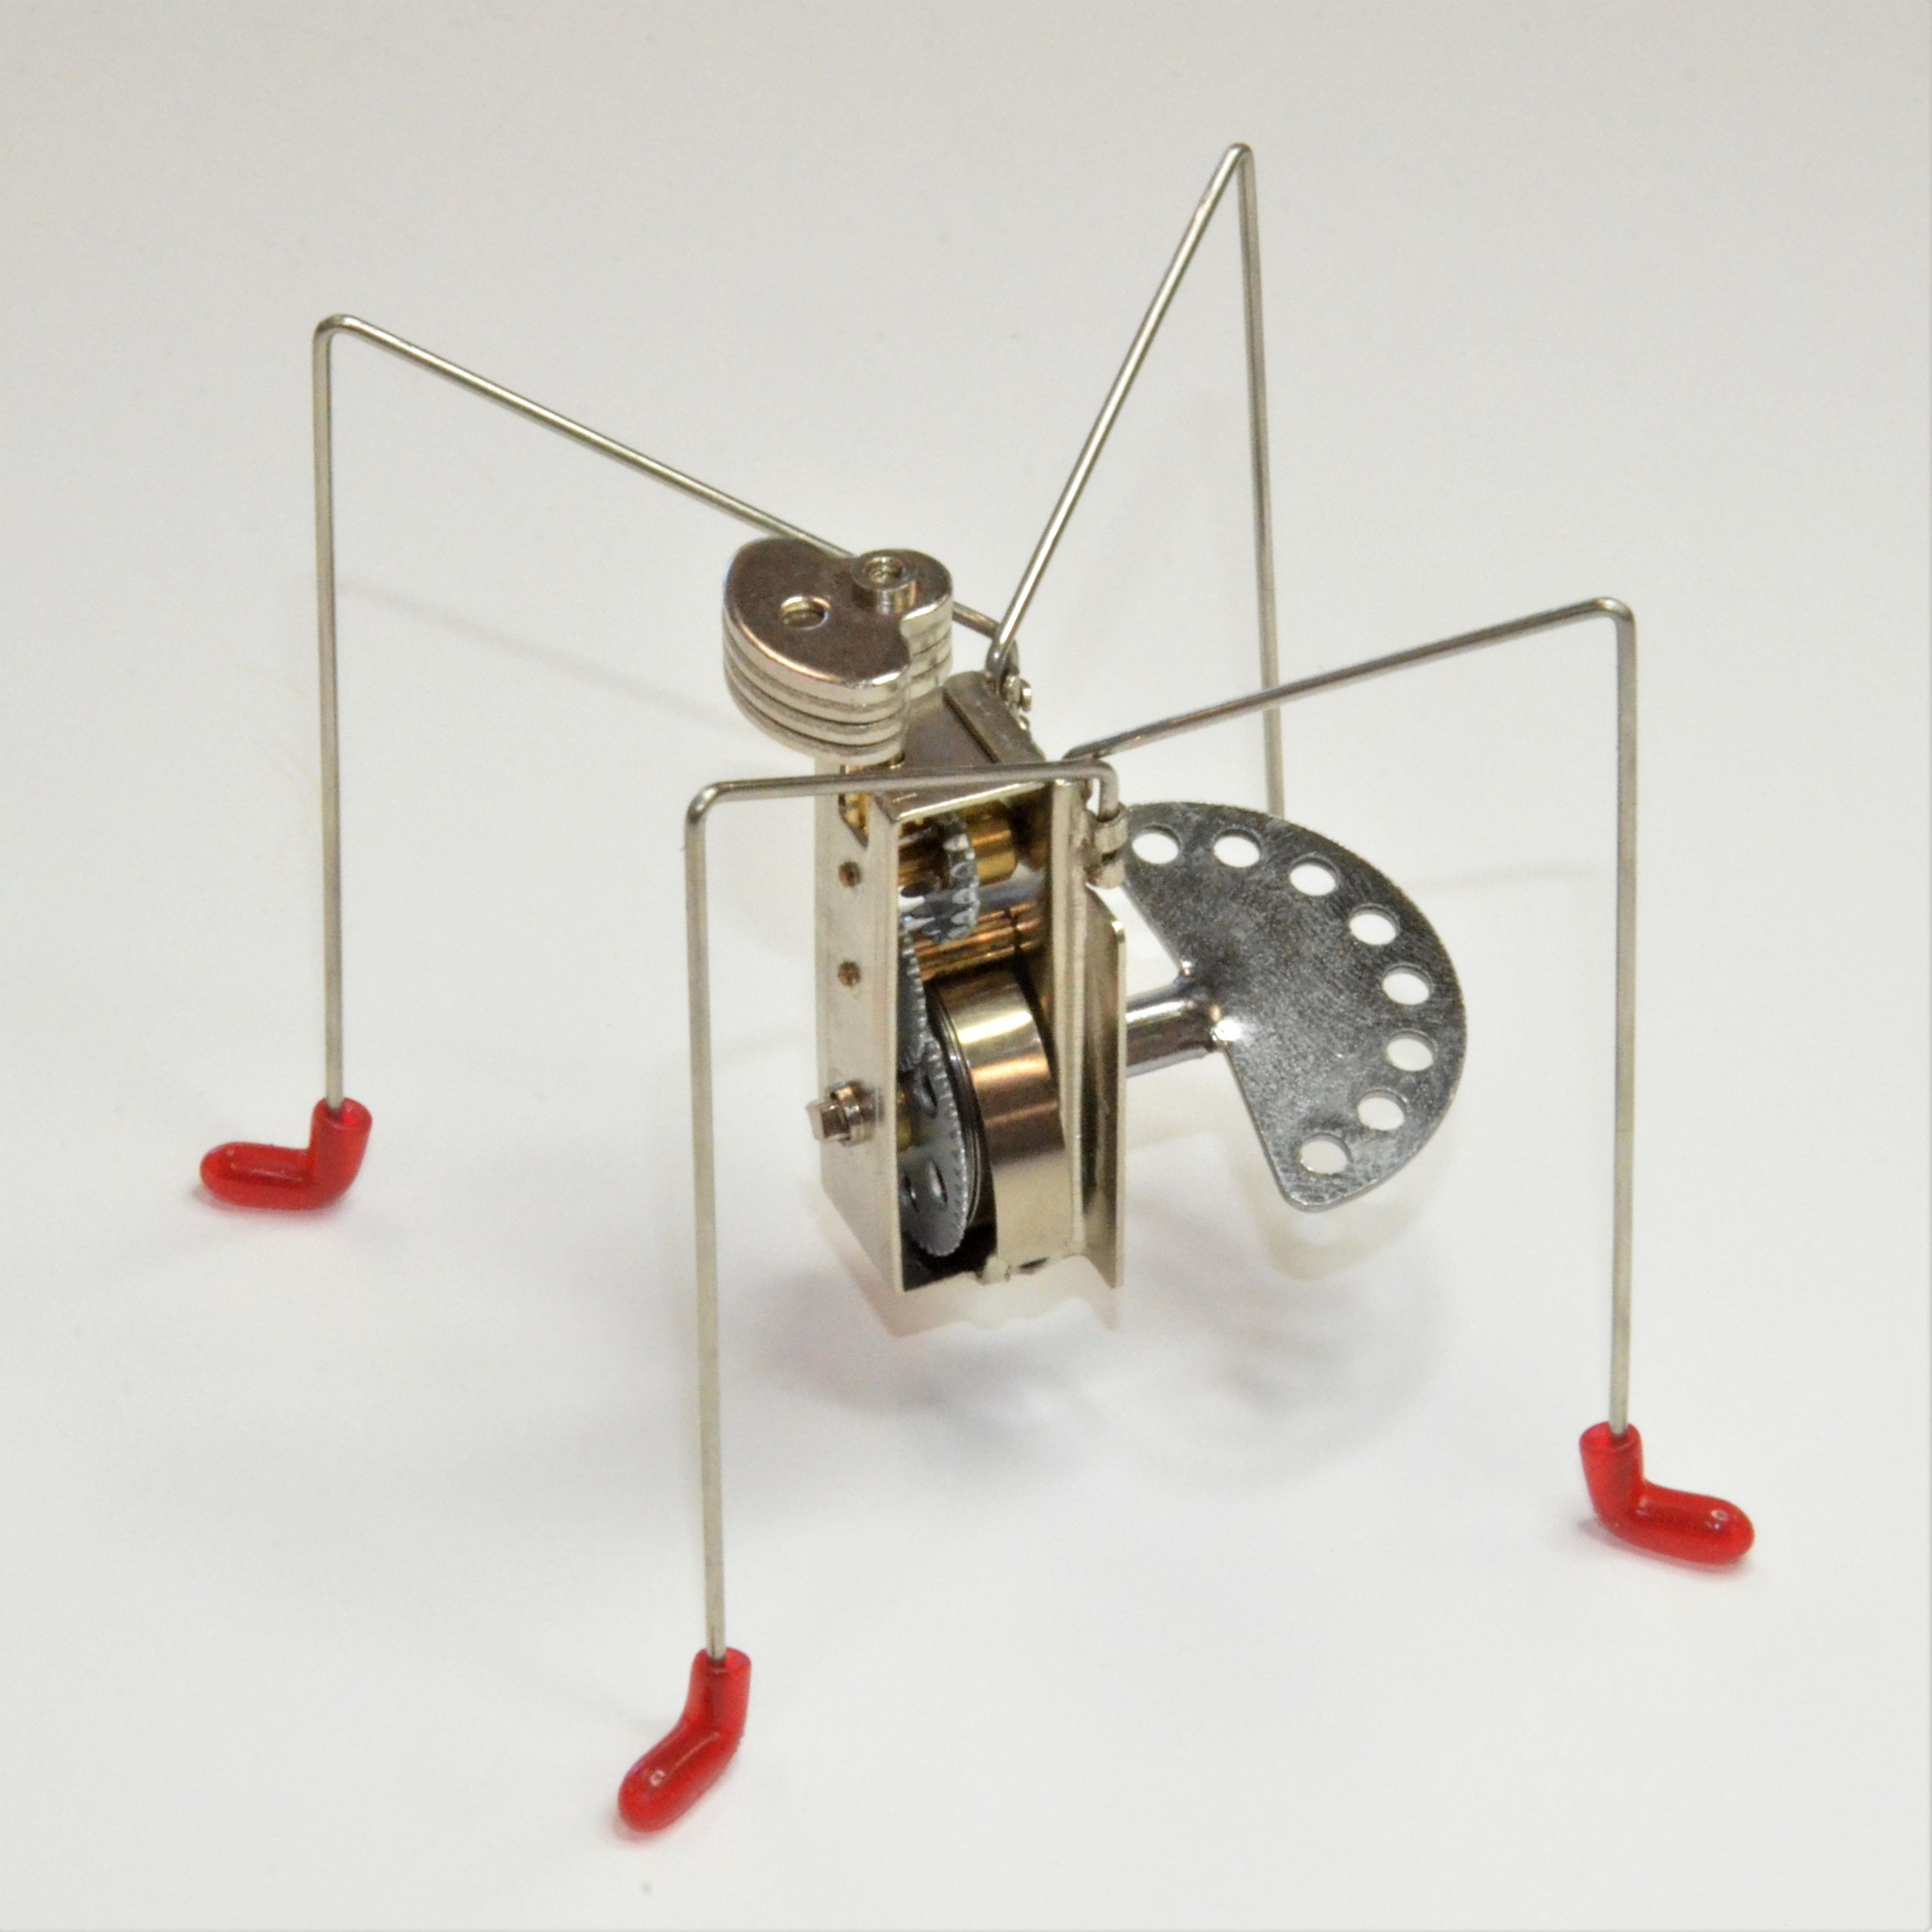
\includegraphics[width=\linewidth]{katita}
    \end{minipage}
    \begin{minipage}[b]{0.49\linewidth}
        \centering
        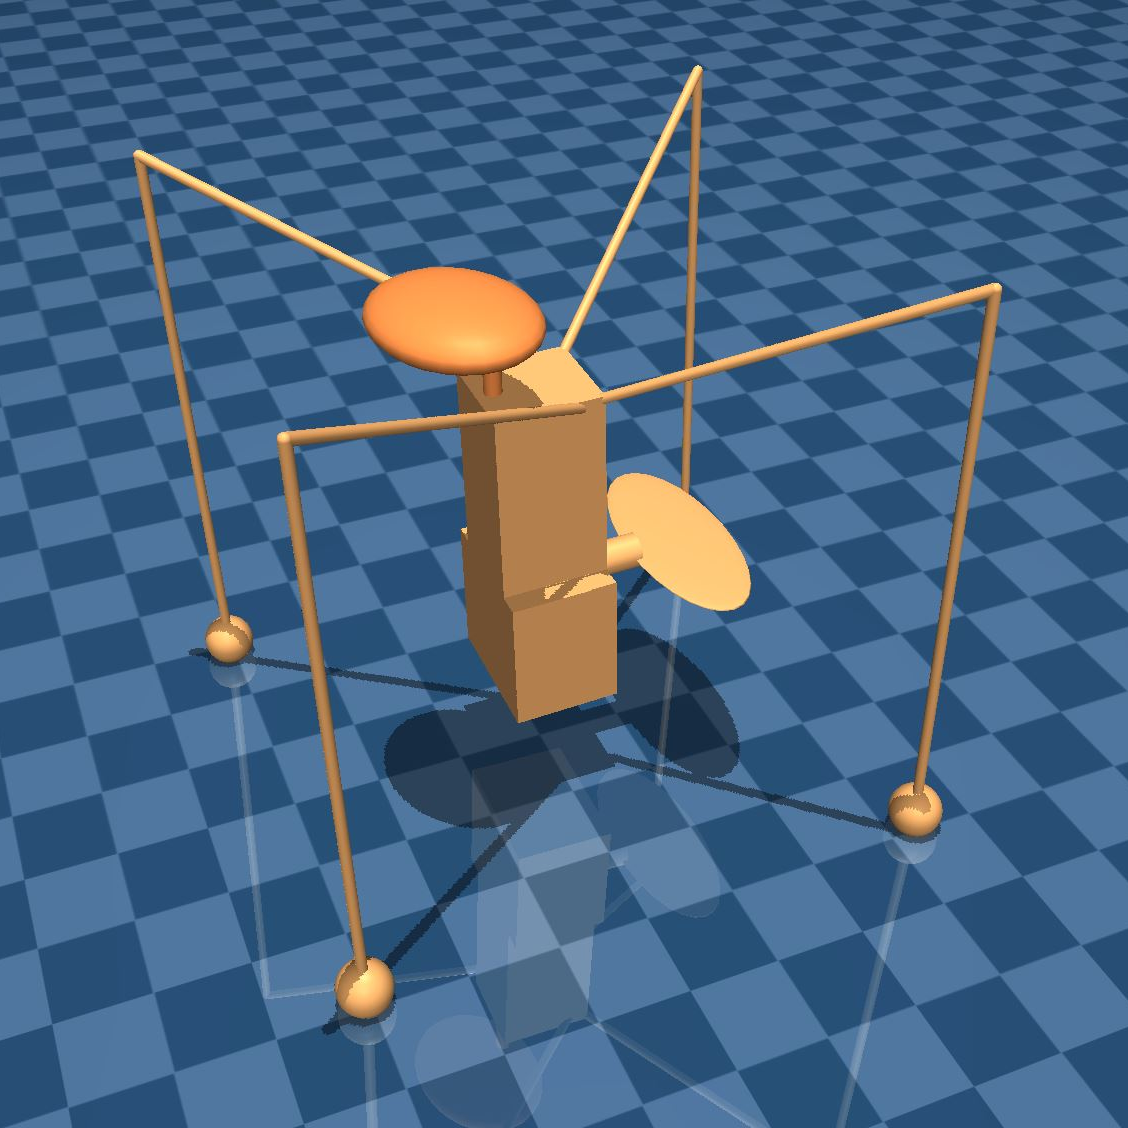
\includegraphics[width=\linewidth]{jitterbug}
    \end{minipage}
    
    \setlength{\belowcaptionskip}{-10pt}
    \caption{
        \textbf{The Jitterbug Problem}: The wind-up children's toy `Katita' (left) was the inspiration for our underactuated `Jitterbug' continuous control task (right).
        In the simulated robot the wind-up spring is replaced with a controlled single degree-of-freedom motor.
        For scale, the blue checks on the simulated floor on the right are 1cm in size.
    }
    \label{fig:leader}
    
\end{figure} 

Interestingly, many robots are underactuated by design, or at times, by circumstance (e.g., due to motor saturation).
Such systems achieve their tasks due to the inherent inter-dependence of their actuation states \cite{spong1998underactuated}.
This implicit structure suggests that an (automatic) reduction of the actuation space may make these systems more compatible with (model-free) Deep Reinforcement Learning methods, which, in turn, would allow for more variable underactuated systems.
Towards this, we introduce a highly variable, single actuator robotic locomotion benchmark (the `Jitterbug' problem) based around a passive compliant toy system with tasks of varying difficulty, particularly around the sparsity of the reward signal (see also Fig.~\ref{fig:leader}).

Reduced order approaches are a common strategy in engineering.
An issue herein is that an under-actuated system, such as the Jitterbug problem, is highly variant in state space and thus difficult to explicitly model in an analytic form.
Note that `highly variable' does not imply `chaotic'; that is, the system is deterministic for over short horizons in the state-space.
However, the motion is clearly non-linear due to the contacts and locomotion phases and gaits (indeed, it has been reported that the Katita toy, on which the problem is based, exhibits a `galloping' locomotion mode \cite{jgn.thesis}).
A nonlinear approach for automatically discovering interesting structure in empirical models is unsupervised learning.
Auto-encoders are a well know neural network approach for this that can automatically discover underlying correlations and their interdependencies \cite{AE_hinton2006reducing}.
In this way, initial (random) exploration helps characterize the implicit structure of the (underactuated) action space that then focuses subsequent Deep Reinforcement Learning control policy learning.

The two contributions of this paper are: (1) a consideration of AutoEncoder-based model reduction for Deep Reinforcement Learning in highly variable, underactuated robot domains; and, (2) the introduction and characterization of the Jitterbug Problem as a diverse underactuated robotics task with dynamic, compliant and non-trivial motion in five scenarios of varying gradations of task complexity.
We find that reduced order models can have similar (reward) performance, yet empirically have less training variance and slightly better learning rates.  
The challenging nature of the Jitterbug task may also help inform future research in automatic controls for flexible robots.

\section{Related Work}

There is a good deal of work, some rather recent, in both the robotics and machine learning communities that is relevant to this work.  The underactuated physical robotics task has the property of continuous states/actions with some correlations between these states.   Thus, the control strategy has to operate over continuous actions, and, ideally, could take advantage of the latent structure. 

\subsection{Deep Reinforcement Learning for Continuous Control}

Reinforcement Learning (RL) methods offer automated tools for controller design of such systems via trail and error \cite{sutton1998reinforcement}, but have been been limited by feature representations and forward models \cite{duan2016benchmarking}. 
Deep Reinforcement Learning algorithms typically address this through the use of deep neural networks for both the policy (`actor') and value function (`critic') which has allowed for operation to the continuous control domain \cite{mnih2015human, DDPG}. 
Such systems may be grouped as using `on-policy' or 'off-policy' learning strategies; where on-policy methods, such as PPO \cite{PPO} and TRPO \cite{TRPO}, are those that use a current policy's action to update the value ($Q$) and off-policy are those methods, such as DDPG \cite{DDPG}, SAC \cite{SAC}, TD3 \cite{TD3}, that update the value via the best action and its total discounted future reward.  

In the context of highly variable, underactuated robotics, on-policy methods may exhibit have lower sample efficiency as they would require new samples to be collected for each gradient step \cite{SAC}.   Conversely, off-policy methods may utilize a replay buffer to minimize correlations between samples \cite{DDPG}, but may have difficulties with brittleness to state-space parameters, stability and convergence \cite{bhatnagar2009convergent}.  In both cases, however, reducing the dimensionality and using a more aligned state-space may reduce these issues. 


\subsection{Reduced Order Approaches for Underactuated Robotics}

Underactuated robots are fundamentally correlated in their actuation space  \cite{tedrake2009underactuated}.
When a model is available control strategies including from optimal control \cite{betts2010practical}, direct collocation \cite{von1993numerical}, and trajectory optimization \cite{kalakrishnan2011stomp} have been applied.
Some novel robots, such as compliant legged robots or soft robots, tend to exhibit complex dynamics that do stymie dynamical system and model reduction approaches as an explicit physical model may not be available \cite{nakajima2015information}.

Given that actuation space for underactuated robots is structured, an autoencoder would be able to automatically discover some of these correlations \cite{AE_hinton2006reducing, ngsparse}.
A concern, however, is that the reduced model is not always intuitive, which would complicate the subsequent synchronization with a model based control strategy.
In this way model-free deep reinforcement learning continuous control methods are rather compatible with an autoencoder's reduced state description.


In the underactuated domain, these ideas have been used to get an empirical model that then inform subsequent model-based control.  For example, Nagabandi, \emph{et al.} \cite{nagabandi2018learning} use a small legged robot in which a neural network forecasts the robot's state at the next timestep which is then used via Model Predictive Control (MPC).  Nishimura, \emph{et al.} use an autoencoder in a similar fashion to inform manipulation with a soft-gripper \cite{nishimura2017thin}.  In both these cases the control model is analytic and the engineering effort is needed to synchronize the empirical model with the controller, which can limit the types of policies and strategies that the robot can learn and execute.  
More generally, model-based methods enjoy sample efficiency, but pose challenges of generalization due the control's model and its assumptions.  

In the machine learning domain, the combination of an autoencoder and deep reinforcement network has been considered for various contexts. 
This has been particularly effective in cases with very high dimensional inputs, such as from video, for low-dimensional independent constraints, such as obstacle locations \cite{finn2016deep, bitzer2010using, lynch2019learning}.  
It has have shown promise in a host of challenging applications including visualmotor learning \cite{finn2016deep} and VR teleoperation \cite{zhang2018deep}. 

The system architecture of this work relates to Lange, \emph{et al.} \cite{lange2010deep} in that we train an autoencoder network, remove the decoder side, and then use the remaining encoder network to compress the input features that are used as part of a Deep Reinforcement Learning control policy search.  In contrast to this work, we do see a benefit with a random policy, sparing the need for a `hint-to-goal' heuristic.  This idea has also been considered more recently by Kimura \cite{kimura2018daqn} for reducing the number of trials during the RL policy training phase.   
Also, in this work, the task is slightly different in that the action space is correlated not only across states, but also across subsequent states in time.  

\section{Method}

\begin{figure}[t]
    \centering
    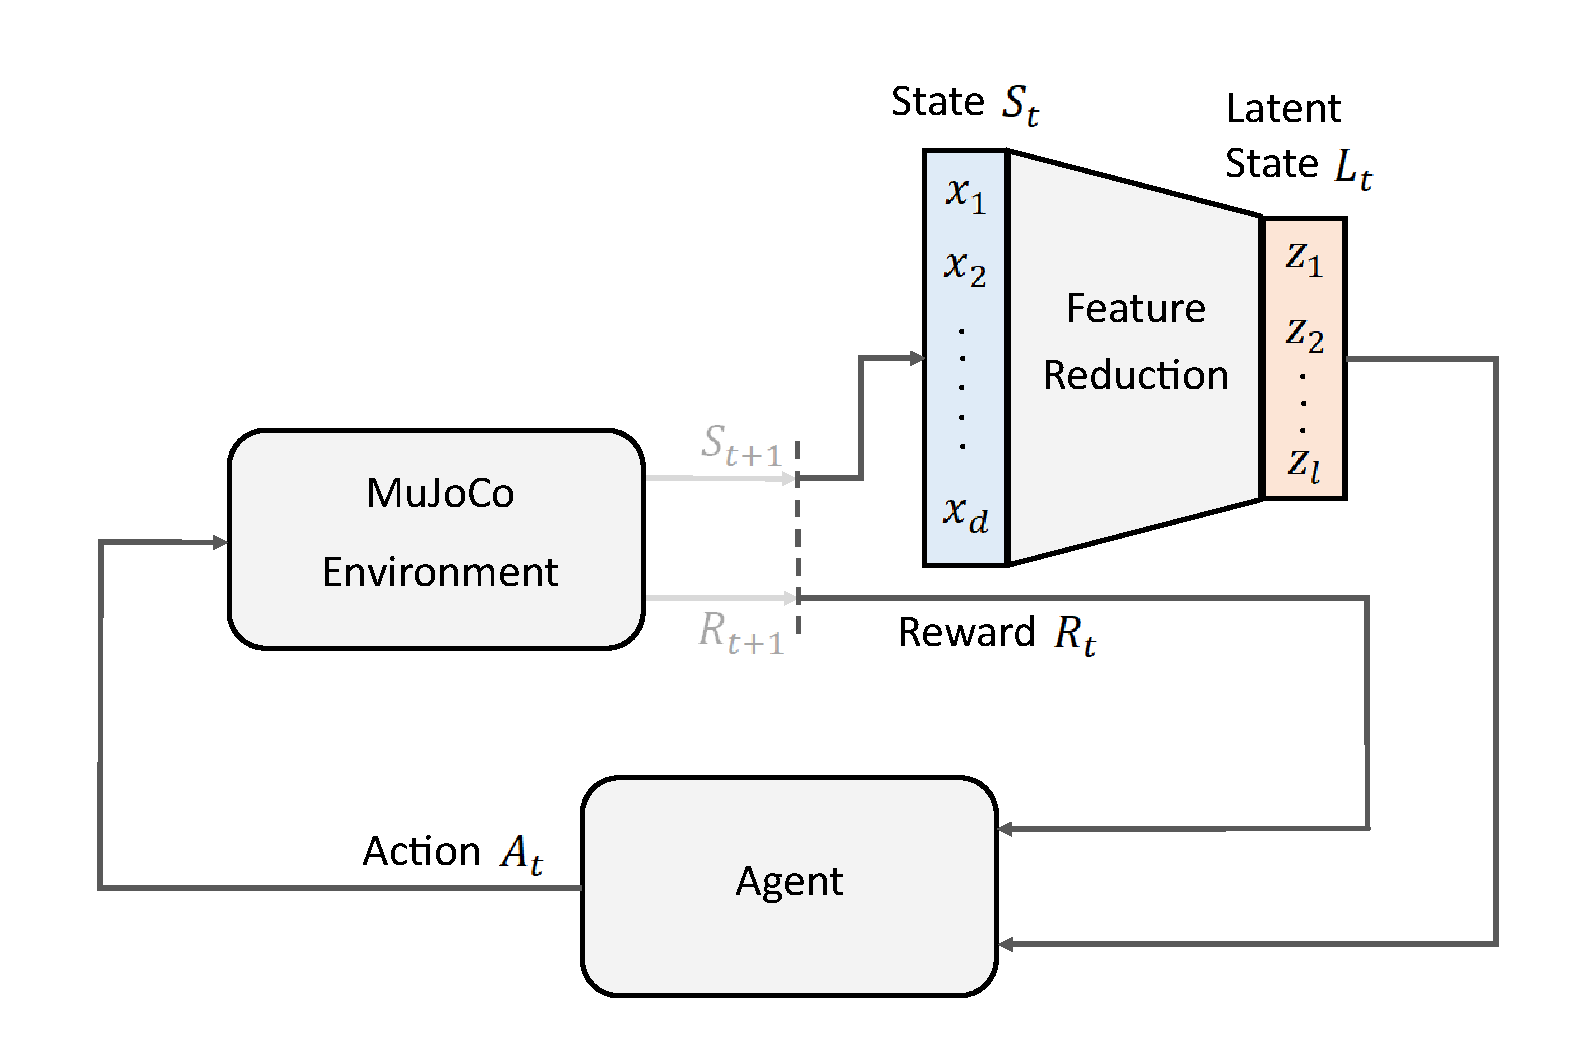
\includegraphics[width=\linewidth]{fig-system-arch}
    \caption{
        \textbf{The architecture of our system.}
    }
    \label{fig:system-arch}
\end{figure}

We use the intuition that an underactuated system has correlations between states %(otherwise it would be uncontrollable for said states)
and thus there is a lower-dimensional representation that could describe this process. 

\hl{Lorem ipsum dolor sit amet, consectetur adipiscing elit. Etiam ultrices nisl at condimentum ultricies. Sed vitae odio magna. Maecenas faucibus volutpat auctor. Nulla facilisi. Etiam aliquam ex nunc, tempus sollicitudin magna dapibus ut. Nulla aliquet felis ante, et dignissim urna viverra sit amet. Aenean aliquet ex id venenatis condimentum. Fusce dui turpis, malesuada non risus vel, vestibulum tincidunt eros.}

\hl{Lorem ipsum dolor sit amet, consectetur adipiscing elit. Etiam ultrices nisl at condimentum ultricies. Sed vitae odio magna. Maecenas faucibus volutpat auctor. Nulla facilisi. Etiam aliquam ex nunc, tempus sollicitudin magna dapibus ut. Nulla aliquet felis ante, et dignissim urna viverra sit amet. Aenean aliquet ex id venenatis condimentum. Fusce dui turpis, malesuada non risus vel, vestibulum tincidunt eros.}


% ------------------------------------------------------------------------------------------------------------------------
\section{A Novel, Underactuated Control Benchmark}
% ------------------------------------------------------------------------------------------------------------------------
We implemented our Jitterbug benchmark using the DeepMind Control Suite (DMC) framework \cite{Tassa2018DMC}.
DMC is a framework and set of benchmark tasks for continuous control published by Google DeepMind in 2018.
DMC benchmarks consist of a \emph{domain} defining a robotic and environment model and \emph{tasks} which are instances of that domain with specific MDP structure

DMC uses the robust Multi-Joint dynamics with Contact (MuJoCo) robotics physics engine for simulation \cite{Todorov2012MuJoCo}.
To aid comparison across tasks, DMC imposes constraints on rewards ($R \in [0, 1]$) and episode length ($H = 1000$).
As such, for any DMC task, cumulative episode return $\approx 1000$ indicates success.

DMC tasks are compatible subsets of the popular OpenAI Gym framework \cite{Brockman2016Gym}, meaning many popular RL algorithm frameworks can be used with these benchmarks.
For our evaluations, we used the \texttt{stable\_baselines} library of RL algorithms \cite{Hill2018Stable}, which is derived from the OpenAI \texttt{baselines} package \cite{Dhariwal2017Baselines}.

\subsection{The Jitterbug Domain}

\begin{figure}[t]
    \centering
    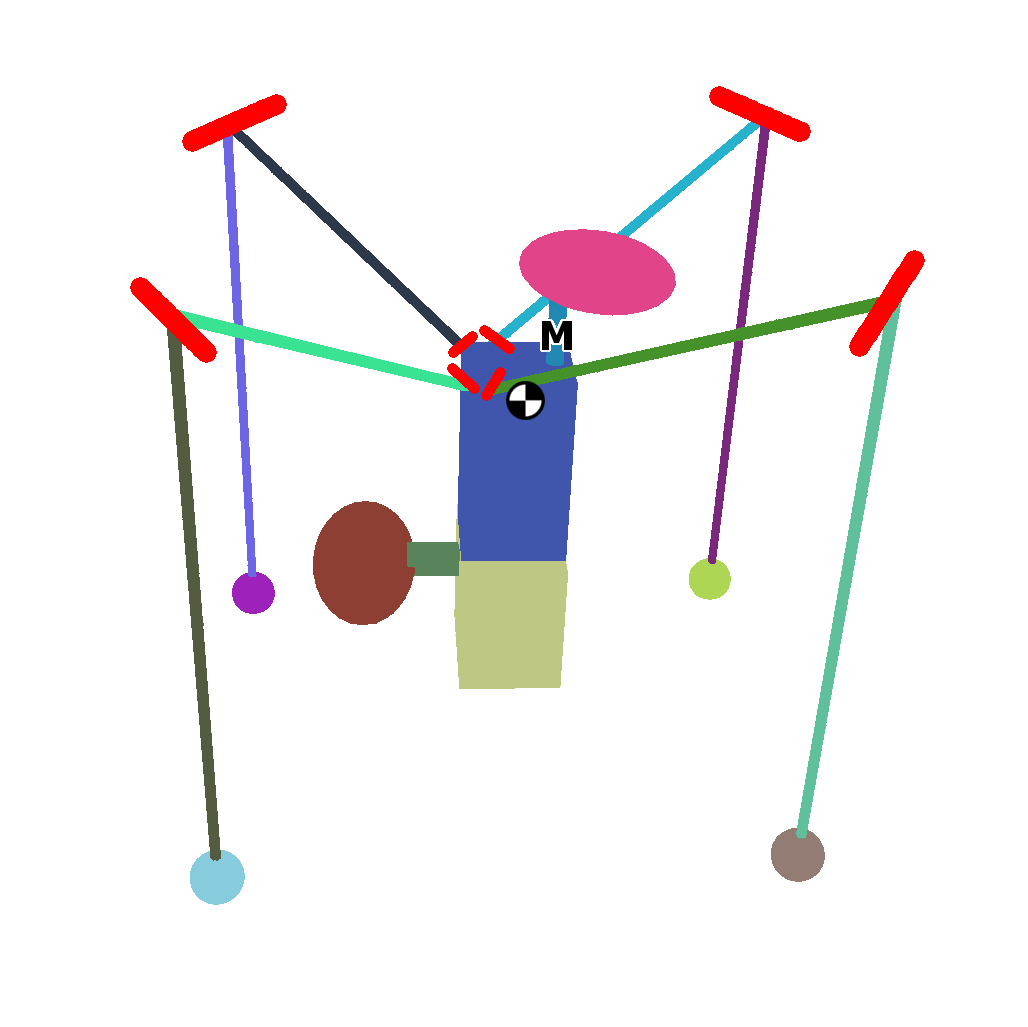
\includegraphics[width=\linewidth]{fig-jitterbug-parts}
    \caption[
        Schematic representation of the Jitterbug model.
        Individual rigid bodies are in different colours and we highlight the position of the center of mass, hinge joints and the single motor.
    ]{
        \textbf{Schematic representation of the Jitterbug model.}
        Individual rigid bodies are in different colours and we highlight the position of the center of mass (\protect\com), hinge joints  (\protect\hinge) and the single motor (\protect\motor).
    }
    \label{fig:parts}
\end{figure}

Our Jitterbug model was inspired by the children's toy Katita (Figure~\ref{fig:leader}).
We aimed to reproduce the physical dynamics of this toy while enabling control by replacing the wind-up spring with a single actuator of equivalent torque.
Our Jitterbug model conforms to the dimensions and mass of the Katita, however we replace the wind-up spring with a controlled single degree-of-freedom torque actuator.
We retain the (non-functional) wind up crank to more closely model the mass distribution of the physical Katita.
Figure~\ref{fig:parts} shows the schematic composition of our simulated Jitterbug model.

We used high-speed recording and visual tachometry to measure the Katita motor speed and leg vibration modes.
By reverse-engineering the Katita gearbox we estimated the torque output of the drive spring and configured the MuJoCo actuator appropriately.
We modelled the legs as rigid bodies with shoulder and elbow hinge joints.
The hinge stiffness was manually tuned to reproduce the dominant leg vibration mode observed in our high-speed footage.
The Jitterbug model density was set using standard values for stainless steel ($7700$ kg/m$^3$) for the body and tough plastic ($1100$ kg/m$^3$) for the feet.

Due to the importance of contact and stiff dynamics in the Jitterbug's locomotion, we found it necessary to adjust MuJoCo's default settings, selecting an integration timestep of 0.0002s and semi-implicit Euler integration.
To simplify the control problem, we use a control timestep of 0.01s.
Thus, one step in the MDP results in 50 steps of the physics simulation and corresponds to 10ms of elapsed time.
Accordingly, an episode (1000 MDP steps) corresponds to 10s of elapsed time.
As is standard practice, during the time between control steps the most recent commanded action is repeated.
With these settings we qualitatively observed a close correspondence between the Katita and the simulated dynamics under constant motor actuation on the Jitterbug.

DMC supports the definition of physically-based camera models to enable learning from raw pixels if desired.
We defined several cameras for the Jitterbug domain including an overhead, tracking and ego-centric view.

\subsection{The Jitterbug Task Suite}

The Jitterbug dynamics naturally induce very high variance motion under a range of motor velocities.
We defined a collection of five tasks of increasing difficulty based on the Jitterbug domain.
The tasks were designed with increasingly sparse reward signals to increase the difficulty.

For all tasks we choose $\gamma = 0.99$ and consider a task solved when cumulative episode reward is $\gtrapprox 900$.
In all tasks the Jitterbug is reset to a random pose near the origin at the start of an episode.
All tasks have a single continuous action controlling the motor $\mathcal{A} = [-1, 1]$ (larger/smaller values are clipped).
All tasks also share the same continuous state space $\text{dim}(\mathcal{S}) = 31$ but differ in the size of the observation space.

For each task, we report ($\text{dim}(\mathcal{O})$) and a brief description of the reward structure.
Tasks are reported here in approximate order of increasing difficulty.

\begin{figure}[t]
    \centering
    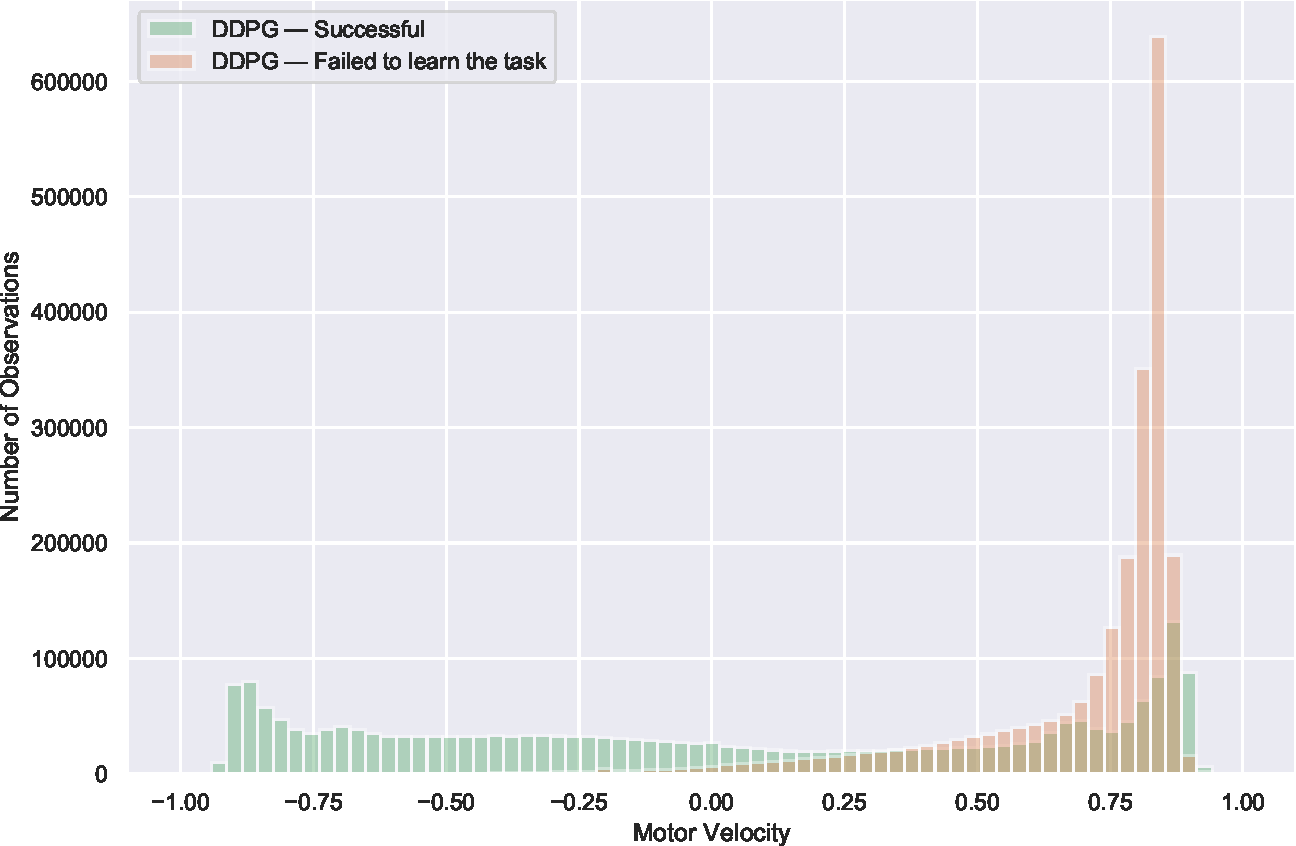
\includegraphics[width=\linewidth]{fig-motor-hist}
    \caption{
        \textbf{Characterising policy behaviours for the \emph{Move In Direction} task.}
        We plot the distribution of motor velocities across many episodes for a successful policy (green) and unsuccessful policy (orange).
        The successful policy learns to pulse the motor in alternating directions as indicated by the spikes near $\pm 1$ in the x-axis.
        Interestingly, this is the same strategy used by our heuristic policies.
        In contrast, the unsuccessful policy gets stuck in a local minima where the motor is continuously driven in one direction.
    }
    \label{fig:motor-hist}
\end{figure}

\begin{figure}[t]
    \centering
    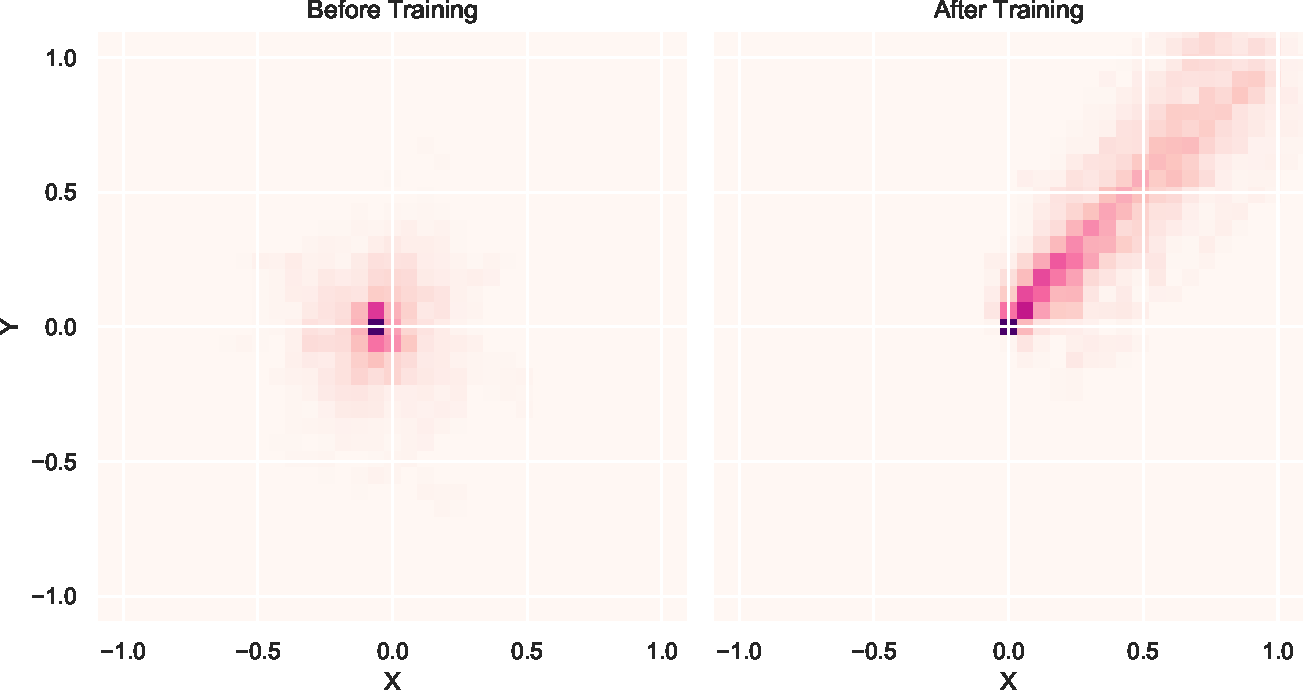
\includegraphics[width=\linewidth]{fig-heatmap}
    \caption{
        \textbf{Heatmap showing Jitterbug position over 100 episodes.}
        The data were collected before (left) and after (right) training DDPG on the task \emph{Move In Direction}.
        In the second figure, to evaluate the agent, the target direction was fixed at $+45\degree$.
    }
    \label{fig:heatmap}
\end{figure}

\begin{enumerate}[topsep=8pt, partopsep=0pt]
    
    \item \emph{Move From Origin} (15): The Jitterbug must move away from the origin in any direction.
    Note that a sufficiently fast constant motor velocity is sufficient to solve this task.
    
    \item \emph{Face In Direction} (16): The Jitterbug must rotate to face in a randomly selected yaw direction.
    
    \item \emph{Move In Direction} (19): The Jitterbug is rewarded for velocity in a randomly selected direction in the X, Y plane.
    
    \item \emph{Move To Position} (18): The Jitterbug must move to a randomly selected position in the X, Y plane.
    
    \item \emph{Move To Pose} (19): The Jitterbug must move to a randomly selected position in the X, Y plane and rotate to face in a randomly selected yaw direction.
    Note that due to the multiplication of position and yaw reward components, this task has a \emph{very} sparse reward signal.
    
\end{enumerate}

In addition, for all tasks the Jitterbug must remain upright to achieve reward.
Falling does not terminate the episode early as the leg dynamics are sufficiently springy that bouncing into the upright pose again can allow recovery from this condition (albeit at the loss of some reward).
Indeed - we observed some learned strategies that appeared to utilize this mode of locomotion!

\section{Experiments}

\begin{table}[t]
    
    \centering
    \caption{
        \textbf{Algorithm hyper-parameters for DDPG and PPO.}
        Bold items were changed from the defaults offered by the \texttt{stable\_baselines} package.
    }
    \label{tab:hyper-params}
    \medskip
    
    {\def\arraystretch{1.2}
        \begin{tabularx}{0.95\linewidth}{$ X ^ c ^ >{\raggedleft\arraybackslash}p{2.5cm}}
            
            \toprule
            
            Parameter & \phantom{abc} & Value \\
            \midrule
            
            \emph{Shared} & & \\[1pt]
            \quad Optimizer & & Adam \cite{Adam} \\
            \rowstyle{\bfseries} \quad Learning Rate (\boldmath$\alpha$) & & 1{\tiny E}\textsuperscript{--4} \\
            \quad Network Architecture(s) & & Fully Connected \\
            \quad Number of Hidden Layers & & 2 \\
            \rowstyle{\bfseries} \quad Hidden Layer Sizes & & [350, 250] \\
            \rowstyle{\bfseries} \quad Activation Functions & & ReLU \\
            [6pt]
            
            \emph{DDPG} & & \\[1pt]
            \rowstyle{\bfseries} \quad Batch Size & & 256 \\
            \quad Training Steps & & 50 \\
            \quad Rollout and Evaluation Steps & & 100 \\
            \rowstyle{\bfseries} \quad Replay Buffer Size & & 1{\tiny E}\textsuperscript{6} \\
            \quad Soft Update Coefficient ($\tau$) & & 1{\tiny E}\textsuperscript{--3} \\
            \quad Parameter Noise & & None \\
            \rowstyle{\bfseries} \quad Action Noise & & Ornstein-Uhlenbeck \\
            \multicolumn{3}{r}{\boldmath$\mu = 0.3, \sigma = 0.3, \theta = 0.15$} \\
            [6pt]
            
            \emph{PPO} & & \\[1pt]
            \rowstyle{\bfseries} \quad Steps / Environment / Update & & 256 \\
            \rowstyle{\bfseries} \quad Entropy Coefficient & & 1{\tiny E}\textsuperscript{--2} \\
            \quad Value Function Coefficient & & 0.5 \\
            \quad Max Gradient Norm & & 0.5 \\
            \quad Bias-Variance Coefficient ($\lambda$) & & 0.95 \\
            \quad Minibatches & & 4 \\
            \quad Policy Clipping Range & & 0.2 \\
            \quad Value Clipping Range & & None \\
            \quad Surrogate Optimization Epochs & & 4 \\
            [6pt]
            
            \bottomrule
            
        \end{tabularx}
    }
    
\end{table}

\subsection{Characterizing Learned Policies}

To verify feasibility, we hand-crafted heuristic policies that can solve each task.
To characterize the difficulty of the Jitterbug task suite, we performed preliminary hyper-parameter tuning to select reasonable settings and trained several RL algorithms on the tasks.

Figure~\ref{fig:rl-perf} reports training curves for example on- and off-policy algorithms.
We contrast the performance of PPO (an on-policy method) and DDPG (an off-policy method).
%We also overlay the performance of our heuristic policies for comparison.
Each figure shows the median and 10\textsuperscript{th} - 90\textsuperscript{th} percentile episode return across 10 different seeds.

Our selected hyper-parameters are reported in Table~\ref{tab:hyper-params}.
For all cases, we used fully-connected neural networks with hidden layers of size 350 and 250 with ReLU activation.
Where applicable, we use separate networks for the actor and critic (i.e. no shared weights).

We ran additional experiments using TRPO, A2C and SAC and observed similar performance to the reported results.
Training curves for these algorithms are not included here for brevity.

To verify the learned policies were sensible (i.e. to confirm the absence of `reward hacking') we qualitatively and quantitatively investigated the exhibited behaviors.

We observed that a key difference between successful and unsuccessful trained policies seemed to be the ability to learn piecewise control functions.
For example, for all tasks but \emph{Move From Origin}, achieving high reward requires careful modulation of the reactive torque applied to the Jitterbug body by the motor counterweight.
One way to achieve this is by pulsing the motor in different directions -- this is the method we use in our heuristic policies.
We observed that successful policies learned to pulse the motor in short bursts in alternating directions (e.g. $\sim180\degree$ at a time), whereas unsuccessful policies would often drive the motor continuously (Figure~\ref{fig:motor-hist}).
In doing so, the successful policies were able to achieve high cumulative episode return, and accomplish the high-level task encoded by the reward (Figure~\ref{fig:heatmap}).

\subsection{Learning Reduced-Order Representations}

\begin{figure}[t]
    \centering
    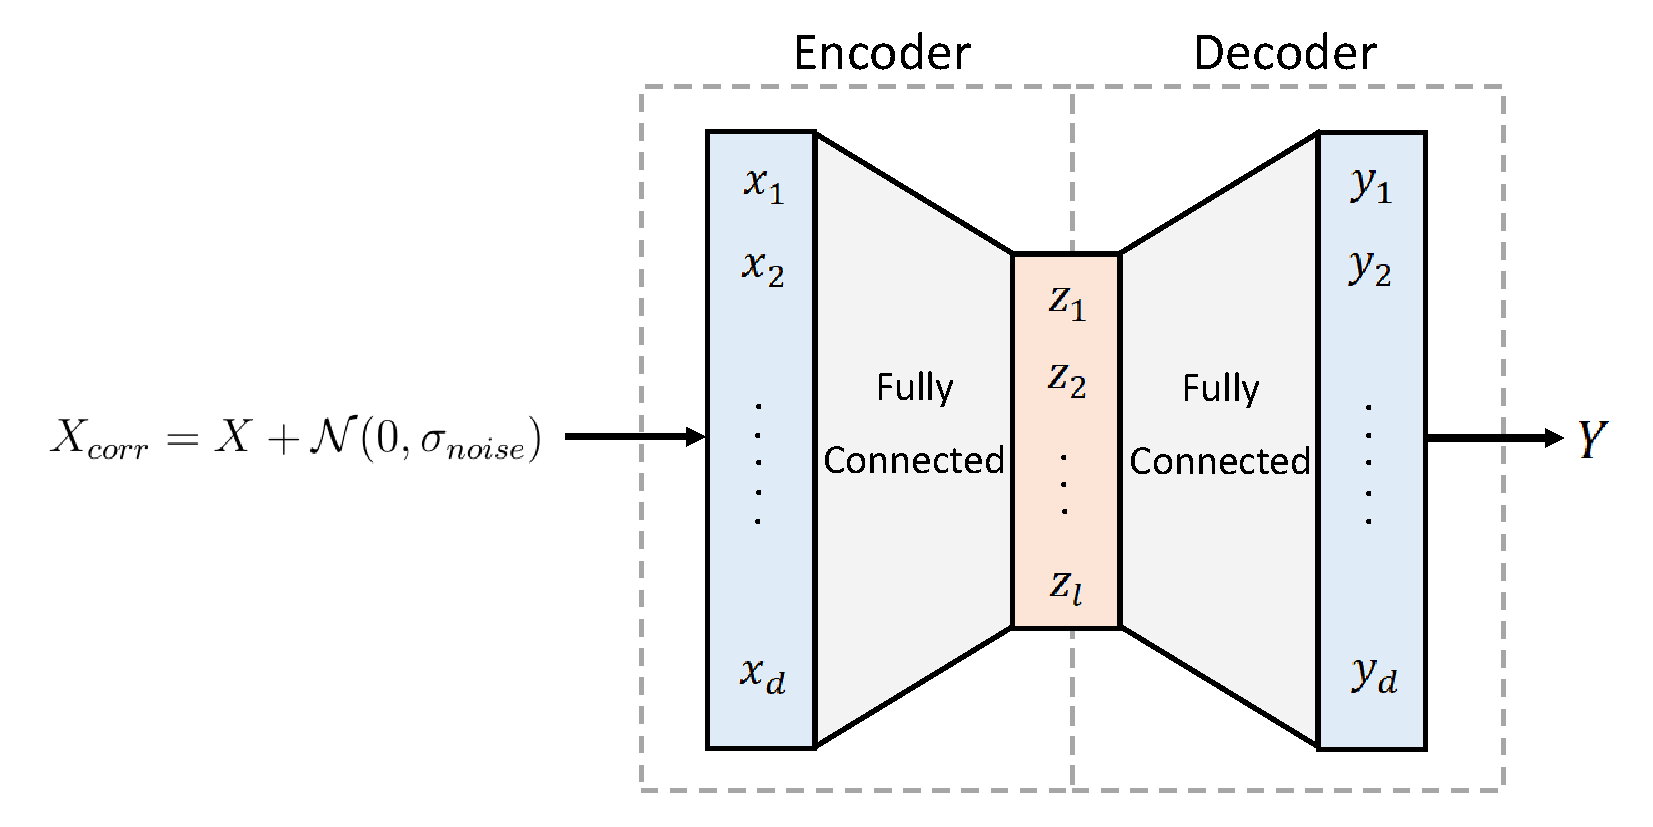
\includegraphics[width=\linewidth]{fig-autoencoder}
    \caption{
        \textbf{Schematic representation of a Denoising AutoEncoder.}
        We use a Denoising AutoEncoder as a means to learn a reduced order observation representation in an unsupervised manner.
    }
    \label{fig:autoencoder}
\end{figure}

We use a De-noising AutoEncoder approach to learn a reduced-order observation representation (Figure~\ref{fig:autoencoder}).
Input states $X$ are corrupted by adding random unbiased noise to each of the features $X_\text{corr} = X + \mathcal{N}(0, 0.1)$.
The AutoEncoder is then trained with input corrupted data $X_{corr}$ and uncorrupted target labels $X$.
We implement this using the mid-level API in the \texttt{tensorflow} library \cite{Abadi2015Tensorflow}.
To optimize the AutoEncoder network we use the Mean Squared Error between the output $Y$ and the original data $X$ as a loss and use the Adam optimizer with default settings \cite{Adam}.

Training data were gathered by running a random policy on the Jitterbug for 5 million steps, and we used 80\% of this data for training and 20\% as a held-out test set.
Once trained, the decoder side of the AutoEncoder was discarded and the encoder used to provide an augmented observation representation to a Deep Reinforcement Learning algorithm.

\subsection{Deep RL with Reduced-Order Representations}

\begin{figure}[t]
    \centering
    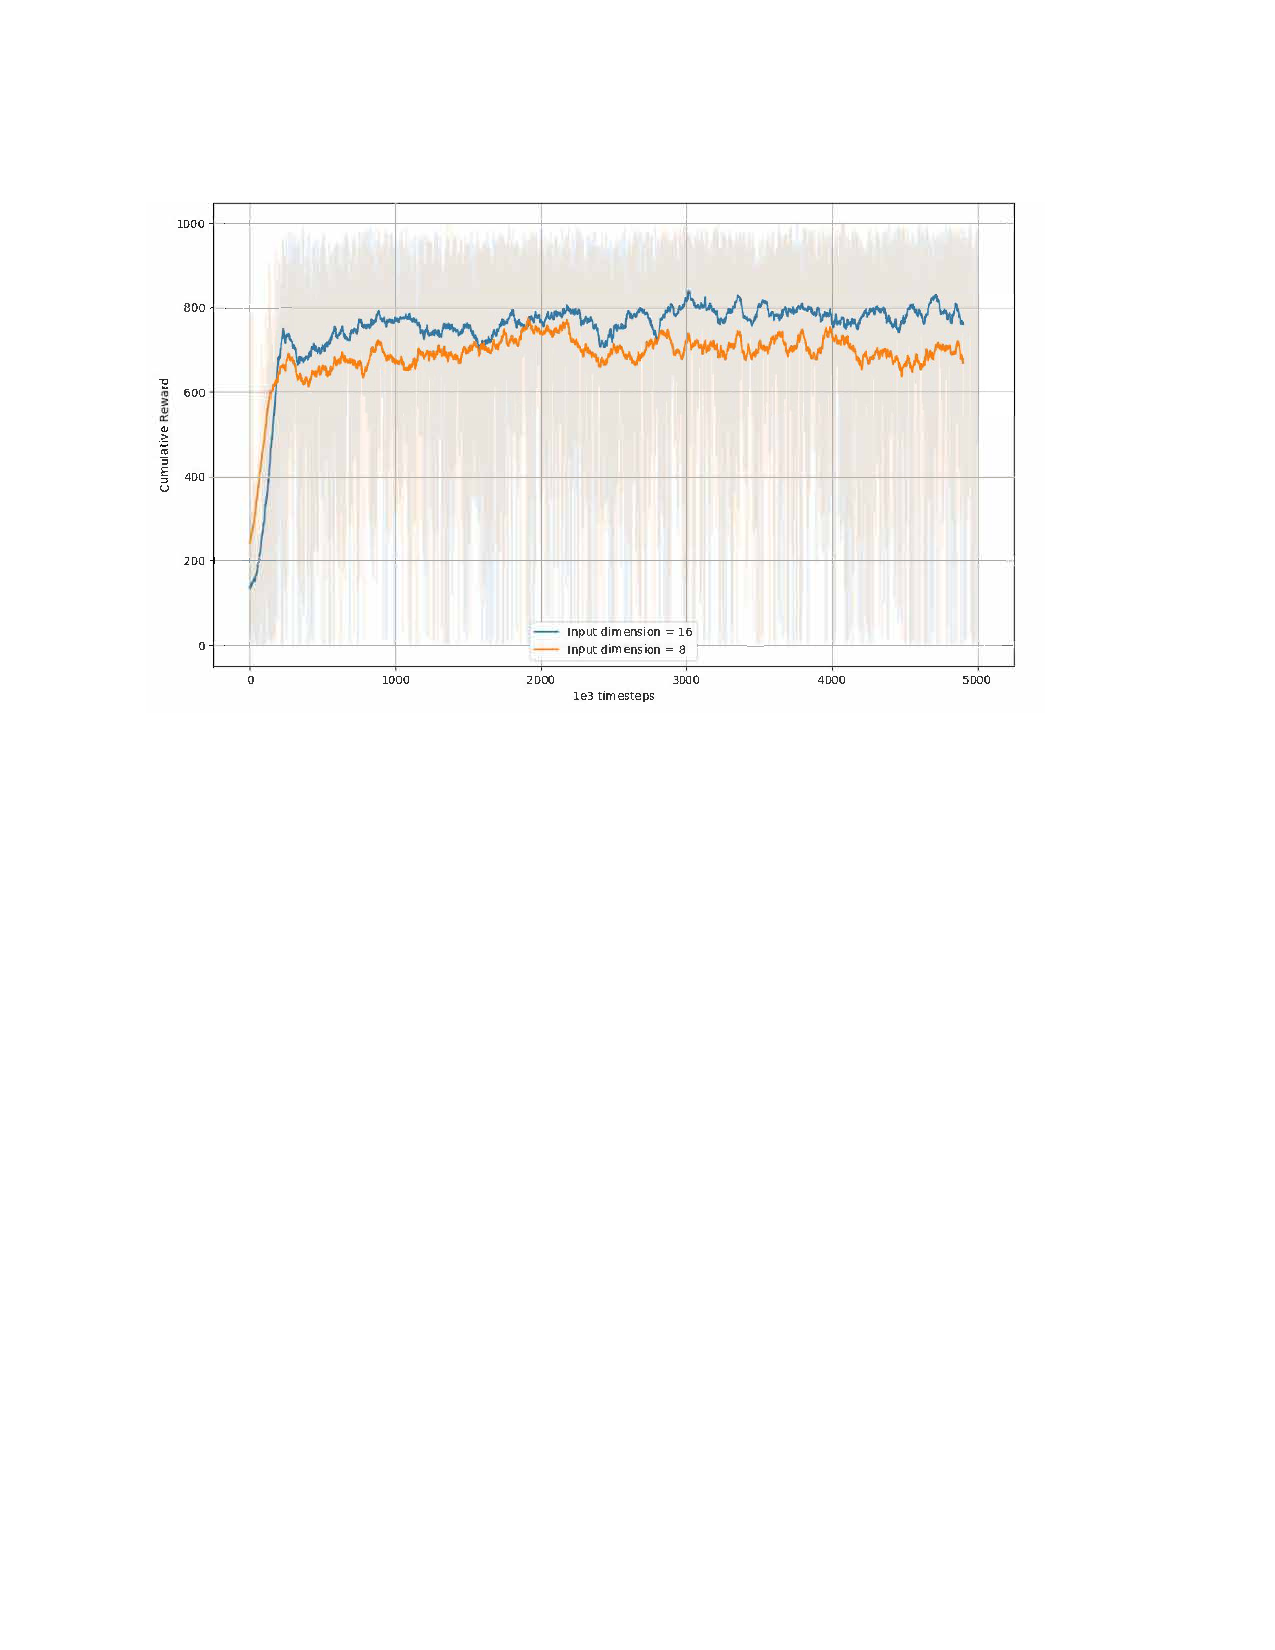
\includegraphics[width=\linewidth]{fig-ae-perf}
    \caption{
        \textbf{Performance of a Deep Reinforcement Learning agent with a reduced-order representation.}
        We plot the training performance of a DDPG agent on the task \textit{Face In Direction} up to 5 million steps.
        Blue: agent with full-order observations (16 dimensions).
        Orange: agent with reduced-order observations from Denoising AutoEncoder (8 dimensions).
        A single random seed is shown and 100-episode moving average filter is applied.
    }
    \label{fig:ae-perf}
\end{figure}

See Figure~\ref{fig:ae-perf}.

\hl{Lorem ipsum dolor sit amet, consectetur adipiscing elit. Etiam ultrices nisl at condimentum ultricies. Sed vitae odio magna. Maecenas faucibus volutpat auctor. Nulla facilisi. Etiam aliquam ex nunc, tempus sollicitudin magna dapibus ut. Nulla aliquet felis ante, et dignissim urna viverra sit amet. Aenean aliquet ex id venenatis condimentum. Fusce dui turpis, malesuada non risus vel, vestibulum tincidunt eros.}

\section{Discussion And Conclusion}

\hl{Lorem ipsum dolor sit amet, consectetur adipiscing elit. Etiam ultrices nisl at condimentum ultricies. Sed vitae odio magna. Maecenas faucibus volutpat auctor. Nulla facilisi. Etiam aliquam ex nunc, tempus sollicitudin magna dapibus ut. Nulla aliquet felis ante, et dignissim urna viverra sit amet. Aenean aliquet ex id venenatis condimentum. Fusce dui turpis, malesuada non risus vel, vestibulum tincidunt eros.}

%\addtolength{\textheight}{-12cm}   % This command serves to balance the column lengths
                                  % on the last page of the document manually. It shortens
                                  % the textheight of the last page by a suitable amount.
                                  % This command does not take effect until the next page
                                  % so it should come on the page before the last. Make
                                  % sure that you do not shorten the textheight too much.

%%%%%%%%%%%%%%%%%%%%%%%%%%%%%%%%%%%%%%%%%%%%%%%%%%%%%%%%%%%%%%%%%%%%%%%%%%%%%%%%

\section*{Acknowledgment}

We thank Dr. Hanna Kurniawati at the ANU Robust Decision-making and Learning Laboratory for discussions and simulation assistance.
This research was partly supported by an Australian Research Council Discovery Project (DP160100714).
A. J. Snoswell is supported in part through and Australian Government Research Training Program Scholarship. 

%%%%%%%%%%%%%%%%%%%%%%%%%%%%%%%%%%%%%%%%%%%%%%%%%%%%%%%%%%%%%%%%%%%%%%%%%%%%%%%%

\bibliographystyle{ieeetr}
\bibliography{root}

\begin{figure*}[p]
    
    \centering
    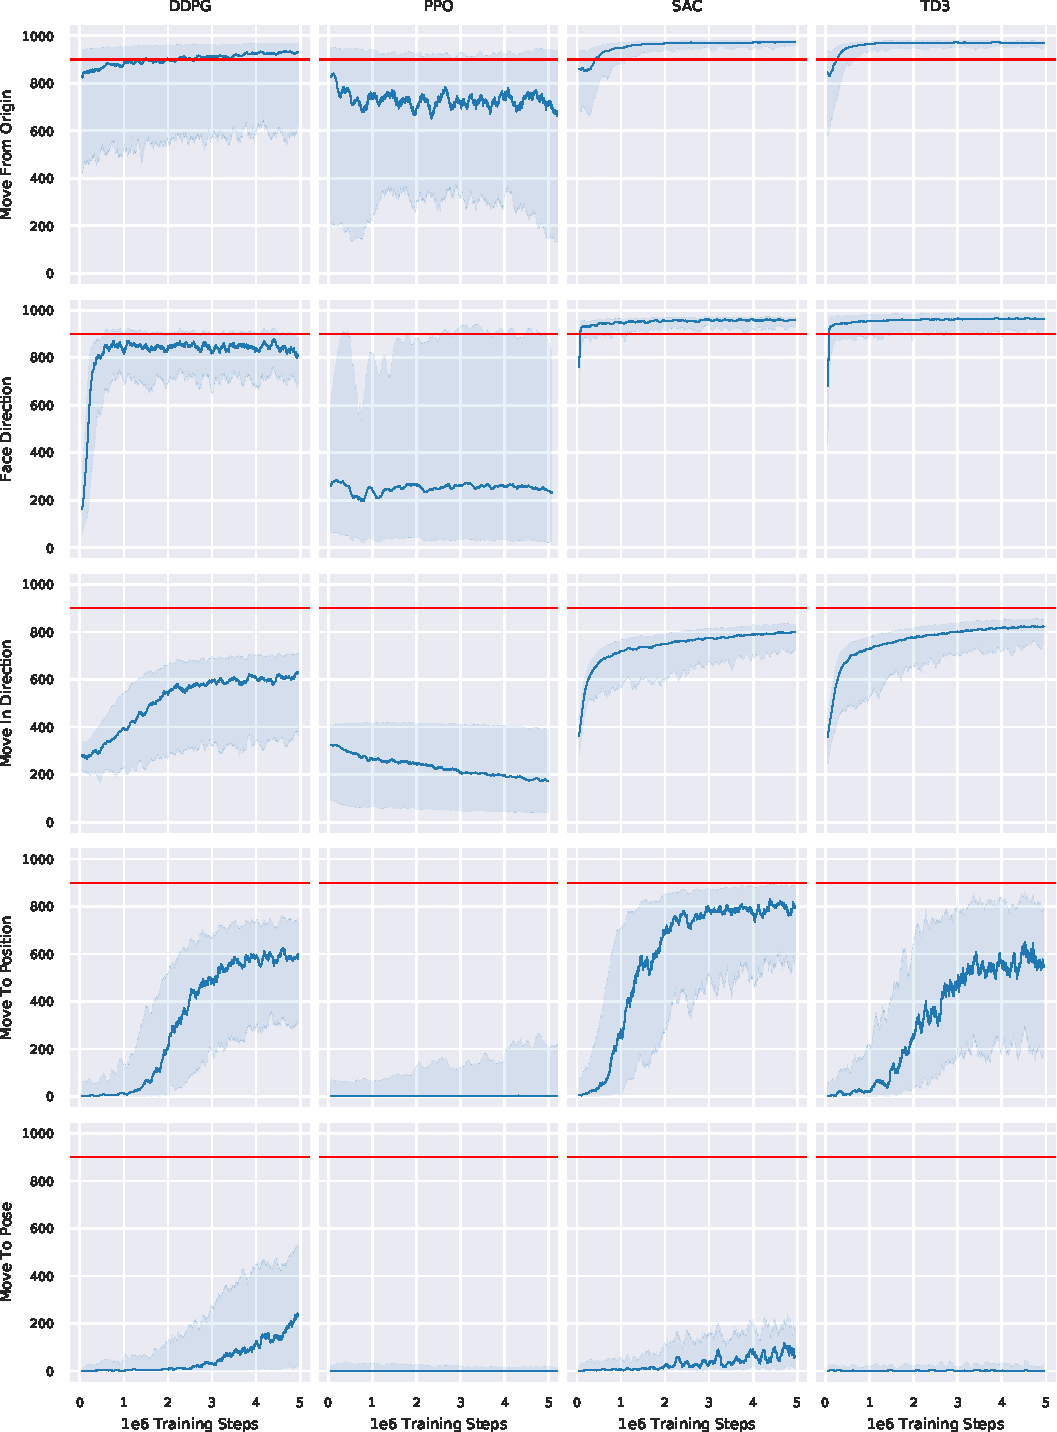
\includegraphics[height=0.94\textheight]{fig-rl-perf}
    
    \caption{
        \textbf{Characterizing the Jitterbug task suite.}
        We compare the training progress of DDPG and PPO up to 5 million training steps (5000 episodes).
        We show median (solid line) and the 10\textsuperscript{th} and 90\textsuperscript{th} quartiles (shaded area) of per-episode episode return across 10 random seeds in each figure.
        A task is considered 'solved' if the trained agent consistently scores $\gtrapprox 900$ return per episode (red line).
        All plots are filtered with a 20{\tiny E}\textsuperscript{3} step moving average filter.
    }
    
    \label{fig:rl-perf}
\end{figure*}

\end{document}
